\documentclass[11pt, a4paper, notitlepage]{report}
\usepackage[dvips]{graphicx,color,rotating}
\usepackage{polski}
\usepackage[utf8]{inputenc}
\usepackage{pstricks}
\usepackage{lipsum}
\usepackage{titling}
\usepackage{appendix}
\usepackage{indentfirst}
\usepackage{float}
\usepackage{caption}

\pretitle{
	\begin{center} 
		\includegraphics[width=40pt,height=40pt]{graphics/znak_pk} \\ 
		 \Huge\bfseries}
\posttitle{\par\end{center}\vskip 0.5em}
\preauthor{\begin{center} \Large  KWD  \\  \LARGE\ttfamily}
\postauthor{ \end{center}}
\predate{\par\large\centering}
\postdate{\par}

\pagestyle{headings}

\author{Piotr Dudek, Mariusz Górny}

\title{\textbf{Przewidywanie stabilności systemu symulującego zmiany klimatyczne (Climate Model Simulation Crashes)}}
\date{29.01.2020}

\pagenumbering{roman} 

\begin{document}
\clearpage\maketitle
\thispagestyle{empty}
\begin{abstract}
Projekt modelu klasyfikatora binarnego dla problemu przewidywania stabilności systemu symulującego zmiany klimatyczne. Baza danych Climate Model Simulation Crusches zawiera informacje na temat parametrów modelu klimatycznego i wyniku o powodzeniu lub niepowodzeniu symulacji. Została przeprowadzona analiza eksploracyjna tych danych, a następnie na ich podstawie, dzięki wykorzystaniu narzędzi do uczenia maszynowego oferowanych przez biblioteki języka Python 3, powstał model klasyfikatora binarnego, który poprawnie przewiduje stabilność systemu. Model wykorzystuje implementację regresji logistycznej, która pozwala na określenie prawdopodobieństwa powodzenia symulacji na podstawie danych wejściowych. Powstałe narzędzie zostało sprawdzone pod kątem jakości dla dostępnych danych.
\end{abstract}

\clearpage \tableofcontents
\thispagestyle{empty}

\setcounter{page}{1}

\chapter{Wprowadzenie}
\pagenumbering{arabic}
Celem projektu jest opracowanie i wytrenowanie modelu klasyfikatora dla problemu przewidywania stabilności systemu symulującego zmiany klimatyczne. Projekt został wykonany za pomocą języka Python 3 z użyciem bibliotek Scikit-learn, Matplotlib i Pandas, służacych do zdefiniowania i~uczenia modelu klasyfikatora, operowania na bazie danych Climate Model Simulation Crashes oraz tworzenia wykresów.

\section{Opis problemu}
Baza danych Climate Model Simulation Crashes zawiera dane parametrów i wyniku o powodzeniu lub niepowodzeniu symulacji, podczas kwantyfikacji niepewności (UQ) modelu klimatycznego. Zestawy wartości 18 parametrów zostały uzyskane metodą łacińskich hiperkostek (ang. Latin Hypercube Sampling (LHS)). Zestawy parametrów zostały wygenerowane w 3 oddzielnych losowaniach, po 180 zestawów parametrów każde. 46 z 540 przeprowadzonych symulacji zakończyło się niepowodzeniem z powodów numerycznych dla konkretnych wartości parametrów. Uzyskany klasyfikator zostanie użyty do przewidywania wyniku symulacji (powodzenia lub niepowodzenia) oraz określenia powodów niepowodzenia symulacji.

\section{Opis danych wejściowych}
Zestaw danych składa się z 540 wierszy, reprezentujących kolejne symulacje. Pierwsza kolumna zawiera numer losowania, za pomocą którego zostały wygenerowane parametry symulacji. Druga kolumna zawiera numer symulacji (od 1 do 180) w obrębie losowania. Kolumny 3-20 zawierają wartości parametrów symulacji, przedstawione w postaci liczby rzeczywistej z przedziału [0, 1]. Ostatnia kolumna zawiera wynik symulacji (0 - niepowodzenie, 1 - powodzenie).
\section{Analiza danych wejściowych}
\begin{figure}[H]
	\centering
	\captionsetup{justification=centering}
	\includegraphics{graphics/data_head}
	\caption{Pierwsze 5 wierszy z bazy danych. Kolumny 4-18 zostały ukryte dla zwiększenia czytelności obrazu.}
\end{figure}
Pierwsze dwie kolumny to dane identyfikujące kolejne symulacje, z tego powodu zostały wyłączone z uczenia i testowania modelu. Ostatnia kolumna zawiera wynik symulacji i została potraktowana jako rezultat dla modelu. Kolumny 3-20 zawierają wartości kolejnych parametrów, które są danymi wejściowymi dla modelu. Wartości te to liczby rzeczywiste z przedziału [0,~1], dlatego nie ma konieczności przeprowadzania dalszej normalizacji danych.\par
Po rozdzieleniu danych na zbiory danych wejściowych i rezultatu, rozmiar tych zbiorów odpowiada opisowi i założeniom:
\begin{verbatim}
	Wymiar danych wejściowych:  (540, 18)
	Wymiar rezultatu:  (540,)
\end{verbatim}
\begin{figure}[H]
	\centering
	\captionsetup{justification=centering}
	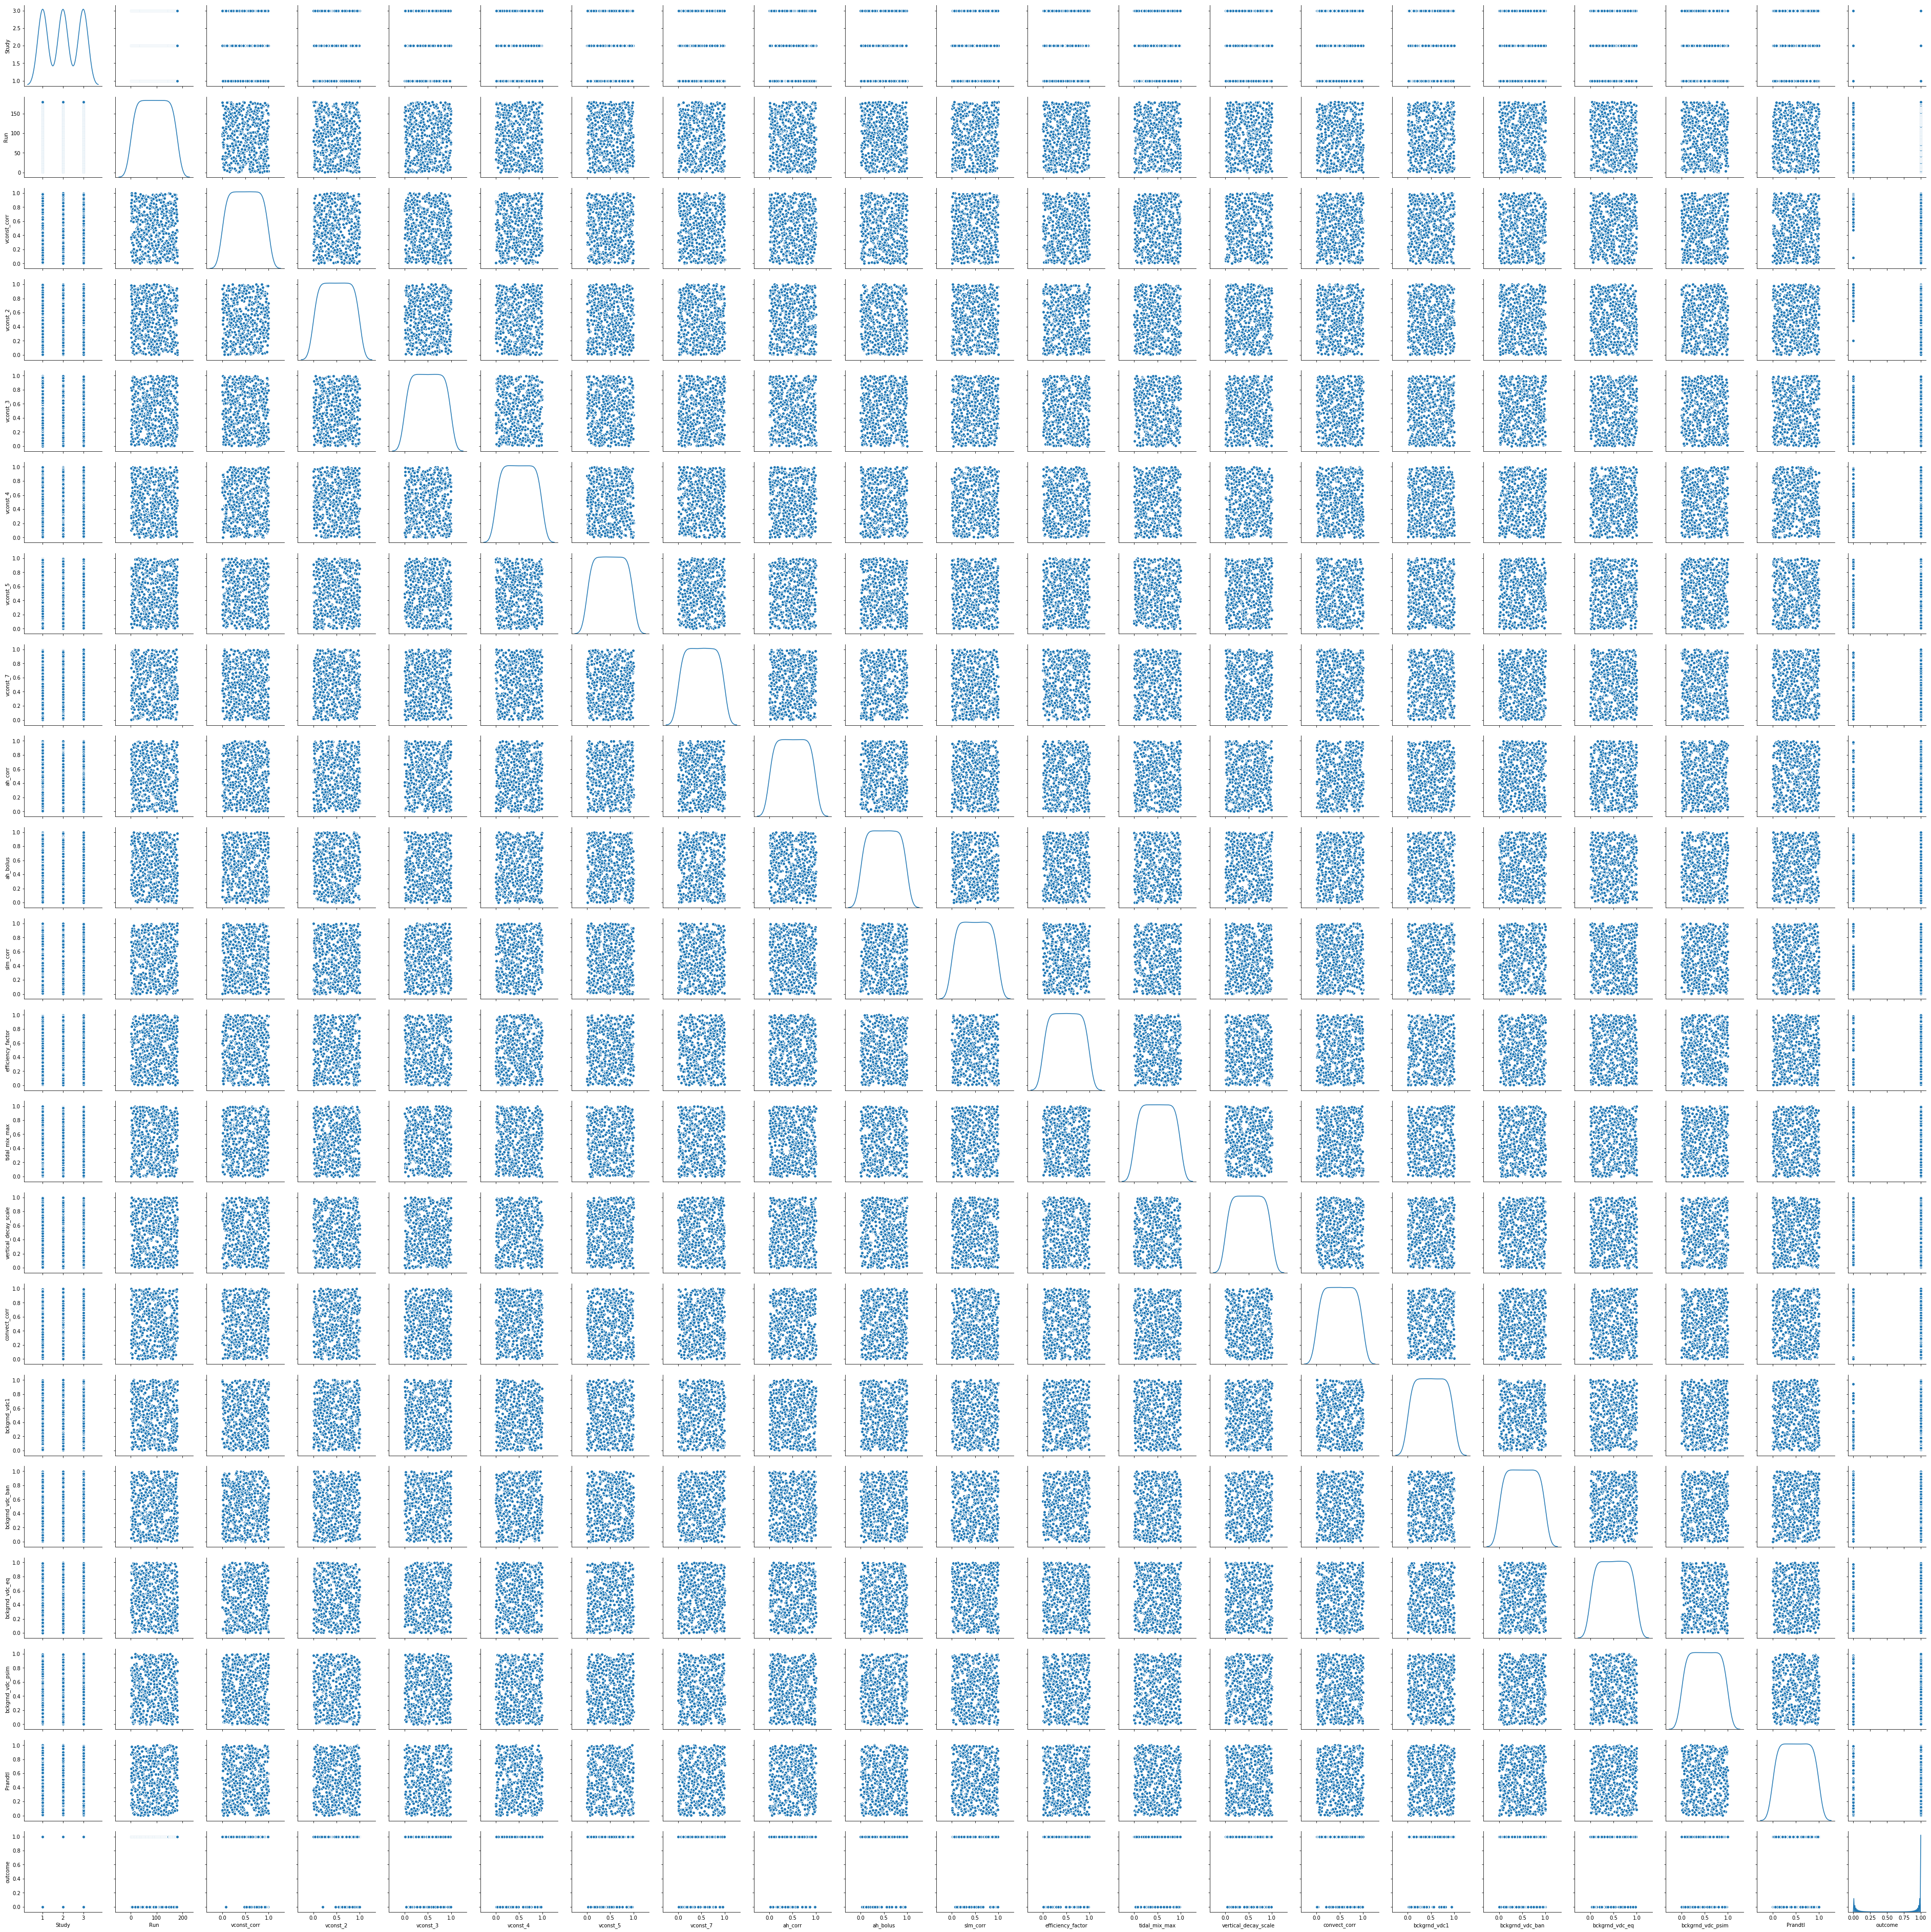
\includegraphics[width=350px]{graphics/wizualizacja}
	\caption{Wynik analizy eksploracyjnej danych.}
\end{figure}\par
Analiza eksploracyjna danych nie wykazała korelacji pomiędzy poszczególnymi wymiarami danych wejściowych. Rozkład wartości parametrów jest inny niż normalny. Jest to spowodowane sposobem uzyskania wartości parametrów - zostały one wygenerowane w taki sposób, aby zestawy parametrów pokrywały całe spektrum możliwych ich wartości. Nie jest możliwa redukcja wymiarów danych wejściowych przed przystąpieniem do tworzenia i trenowania modelu.

\chapter{Opis metody}
\section{Wprowadzenie teoretyczne}
Problem jest przykładem klasyfikacji binarnej, w której dla n-wymiaro-wych danych wejściowych, wynikiem jest prawdopodobieństwo przypisania do jednej z 2 grup (w badanym przypadku - powodzenie (1) lub niepowodzenie (0) symulacji).\par
Wytrenowany model został oparty o regresję logistyczną, liniowy model klasyfikacji binarnej (może być także użyty do klasyfikacji multiklasowej), w którym prawdopodobieństwo przydzielenia do klasy jest uzyskiwane przy pomocy funkcji logistycznej.\par
Regresję logistyczną implementuje klasa \verb|LogisticRegression| z biblioteki Sklearn.

\section{Badania symulacyjne}
Dane wejściowe i rezultat zostały rozdzielone na zbiory testowy i~uczący w stosunku 1 do 9. Następnie przy pomocy GridSearchCV, z zastosowaniem różnych wartości parametrów: \verb|C|, \verb|penalty|, \verb|max_iter| oraz \verb|tol|, został znaleziony najoptymalniejszy zestaw parametrów dla regresji logistycznej:\par
\begin{verbatim}
	Najlepszy model został znaleziony dla parametrów 
	{'C': 100.0, 'max_iter': 100, 'penalty': 'l2', 'tol': 0.0001} 
	ze współczynnikiem determinacji: 0.9526748971193416.
\end{verbatim} \par
\section{Analiza jakości modelu}
\begin{figure}[H]
	\centering
	\captionsetup{justification=centering}
	\includegraphics[width=200px]{graphics/conf_matrix}
	\caption{Matryca konfuzji dla wytrenowanego modelu.}
\end{figure}\par
Matryca konfuzji wykonana dla danych testowych pokazuje, że model bardzo dobrze przewiduje wyniki powodzenia symulacji. W celu lepszej oceny modelu została przeprowadzona walidacja krzyżowa (\verb|cross_val_score|) z 3, 5, 7 i 10 podziałami (wartość parametru \verb|cv|). Wynik walidacji przedstawia rysunek 2.2:\par
\begin{figure}[H]
	\centering
	\captionsetup{justification=centering}
	\includegraphics[width=290px]{graphics/cross_val}
	\caption{Wykres wartości współczynnika determinacji dla poszczególnych podziałów walidacji krzyżowej.}
\end{figure}\par
Nawet dla bardzo różnych podziałów bazy danych, model utrzymuje wysoki współczynnik determinacji - powyżej 0,92. Podczas uczenia modelu nie zaszło także zjawisko overfittingu, dzięki czemu model powinien poprawnie przewidywać wynik symulacji modelu klimatycznego dla nowych zestawów wartości parametrów.

\chapter{Podsumowanie}
Cel projektu został osiągnięty. Analiza zbioru danych Climate Model Simulation Crashes nie wykazała korelacji pomiędzy poszczególnymi parametrami modelu klimatycznego, przez co nie było możliwe wyodrębnienie parametrów nieistotnych.\par 
Do rozwiązania problemu został zastosowany kwalifikator binarny - regresja logistyczna. Po dobraniu odpowiednich parametrów dzięki zastosowaniu procedury GridSearch, pozwoliła ona na stworzenie modelu poprawnie przewidującego stabilność systemu symulującego zmiany klimatyczne. Powstałe narzędzie zostało sprawdzone pod kątem jakości rozwiązania - współczynnik determinacji po walidacji krzyżowej zawiera się w przedziale 0,92 - 1,0. Model spełnia założenia projektu i może być przydatny do dalszych badań nad systemem symulującym zmiany klimatyczne.

\begin{appendices}
\chapter{Kod programu}
\begin{verbatim}
import pandas as pd
import numpy as np
import matplotlib.pyplot as plt
from sklearn.model_selection import train_test_split
from sklearn.model_selection import GridSearchCV
from sklearn.model_selection import cross_val_score
from sklearn.linear_model import LogisticRegression
from sklearn.metrics import confusion_matrix
import seaborn as sb
	
#wczytanie danych z pliku CSV
pd_data = pd.read_csv('pop_failures.csv')

#wyświetlenie pierwszych wierszy danych
pd_data.head()

#wyodrębnienie danych wejściowych i rezultatu
target = np.array(pd_data["outcome"])
data = np.array(pd_data.iloc[:,2:-1].values)

#wyświetlenie rozmiaru danych
print("Wymiar danych wejściowych: ", data.shape)
print("Wymiar rezultatu: ", target.shape)

#wizualizacja danych
sb.pairplot(pd_data, diag_kind="kde")

#rozdzielenie danych na zbiory uczący i testowy
train_data, test_data, train_target, test_target = \
train_test_split(data,target, test_size=0.1, random_state=1)

#wyszukanie najoptymalniejszego modelu regresji logistycznej
logistic_regression_gs = GridSearchCV(
    LogisticRegression(),
    {
        "C": np.logspace(-3,3,7), 
        "penalty": ["l1","l2"],
        "max_iter": [100, 500, 1000],
        "tol": [1e-4, 1e-5, 1e-6]
    },
    cv=10)
logistic_regression_gs.fit(train_data,train_target)

print("Najlepszy model został znaleziony dla parametrów", \ 
    logistic_regression_gs.best_params_, \
    "ze współczynnikiem determinacji:", \ 
    logistic_regression_gs.best_score_)

#matryca konfuzji dla wytrenowanego modelu
sb.heatmap(confusion_matrix(test_target, \
    logistic_regression_gs.predict(test_data)), \ 
        annot=True, cmap="Blues")

#ocena jakości modelu z zastosowaniem walidacji krzyżowej
cvs = [3, 5, 7, 10]
results = []
for cv in cvs:
    results.append( \
        cross_val_score(logistic_regression_gs, \ 
            data, target, cv=cv))
	
#wyświetlenie wyniku walidacji krzyżowej
markers = ['r-', 'g-.', 'b:', 'y--']
for i in range(4):
    plt.plot([x / (cvs[i]+1) for x in range(cvs[i])], \
        results[i], markers[i], label='cv='+str(cvs[i]))
plt.legend()
plt.ylim(0.9, 1)
plt.gca().xaxis.set_visible(False)
plt.ylabel('wspł. determinacji')
plt.show()
\end{verbatim}
\end{appendices}

\end{document}